\begin{question}[ID=1.1, subtitle={Flusso magnetico attraverso superficie rettangolare}, tags={induzione magnetica, flusso}, difficulty=facile]
Un campo magnetico uniforme $B = 2\ \text{T}$ attraversa una superficie rettangolare di dimensioni $3\ \text{m}\times 4\ \text{m}$.
\begin{enumerate}
    \item Calcola il flusso magnetico $\Phi_B$ quando il campo è perpendicolare alla superficie.
    \item Calcola il flusso quando l'angolo tra $\vec{B}$ e la normale alla superficie diventa $\theta = 60^\circ$.
\end{enumerate}
\begin{solution}
    \begin{enumerate}
        \item Il flusso magnetico è il prodotto del campo per l'area attraversata, quando il campo è perpendicolare alla superficie (parallelo alla normale):
        \[
        \Phi_B = B\,A = 2\cdot 12 = \mathbf{24\ \text{Wb}}.
        \]
        \item In generale conta solo la componente del campo lungo la normale, cioè $B\cos\theta$:
        \[
        \Phi_B = B\,A\cos 60^\circ = 24\cdot 0{,}5 = \mathbf{12\ \text{Wb}}.
        \]
    \end{enumerate}
\end{solution}
\end{question}

%-----------------------------------------------%
\begin{question}[ID=1.2, subtitle={f.e.m. e corrente indotta in circuito con campo variabile linearmente}, tags={induzione magnetica, legge di Faraday}, difficulty=facile]
Un circuito rettangolare di resistenza $R = 5\ \Omega$ e area $A = 0{,}2\ \text{m}^2$ è immerso in un campo magnetico perpendicolare che cresce nel tempo secondo $B(t) = 0{,}4\,t$ (in tesla).
\begin{enumerate}
    \item Calcola la forza elettromotrice indotta.
    \item Calcola la corrente indotta al tempo $t = 5\ \text{s}$.
\end{enumerate}
\begin{solution}
    \begin{enumerate}
        \item Per la legge di Faraday-Neumann, la f.e.m. indotta è l'opposto della rapidità di variazione del flusso. Con area costante, $\Phi = AB(t)$ e $\dfrac{dB}{dt} = 0{,}4\ \text{T/s}$:
        \[
        \mathcal{E} = -A\,\frac{dB}{dt} = -0{,}2\cdot 0{,}4 = \mathbf{-0{,}08\ \text{V}}.
        \]
        \item La corrente segue dalla legge di Ohm. Poiché $dB/dt$ è costante, la f.e.m. (e quindi la corrente) non dipende dall'istante considerato:
        \[
        I = \frac{|\mathcal{E}|}{R} = \frac{0{,}08}{5} = \mathbf{0{,}016\ \text{A}}.
        \]
    \end{enumerate}
\end{solution}
\end{question}

%-----------------------------------------------%
\begin{question}[ID=1.3, subtitle={Solenoide con campo variabile — flusso totale e f.e.m. indotta}, tags={induzione magnetica, solenoide}, difficulty=media]
Un solenoide è lungo $l = 0{,}5\ \text{m}$, ha $N = 100$ spire di raggio $r = 0{,}1\ \text{m}$ ed è percorso da un campo $B = 0{,}3\ \text{T}$.
\begin{enumerate}
    \item Calcola il flusso magnetico totale concatenato.
    \item Calcola la f.e.m. indotta se il campo varia con $dB/dt = 2\ \text{T/s}$.
\end{enumerate}
\begin{solution}
    \begin{enumerate}
        \item Il flusso totale è il flusso attraverso una spira moltiplicato per il numero $N$ di spire. L'area di una spira è $A = \pi r^2 = \pi\cdot 0{,}01 = 0{,}03142\ \text{m}^2$, quindi
        \[
        \Phi_{tot} = N\,B\,A = 100\cdot 0{,}3\cdot 0{,}03142 \approx \mathbf{0{,}942\ \text{Wb}}.
        \]
        \item La f.e.m. indotta in un solenoide è proporzionale al numero di spire:
        \[
        \mathcal{E} = -N\,A\,\frac{dB}{dt} = -100\cdot 0{,}03142\cdot 2 \approx \mathbf{-6{,}28\ \text{V}}.
        \]
    \end{enumerate}
\end{solution}
\end{question}

%-----------------------------------------------%
\begin{question}[ID=1.4, subtitle={Spira circolare in campo B(t) = 3t² — f.e.m. e corrente a t=2 s}, tags={induzione magnetica, Faraday}, difficulty=media]
Una spira circolare di raggio $r = 0{,}2\ \text{m}$ e resistenza $R = 10\ \Omega$ è immersa in un campo magnetico perpendicolare $B(t) = 3t^2$ (in tesla).
\begin{enumerate}
    \item Calcola la f.e.m. indotta a $t = 2\ \text{s}$.
    \item Calcola la corrente indotta nello stesso istante.
\end{enumerate}
\begin{solution}
    \begin{enumerate}
        \item Qui il campo varia in modo non lineare, quindi $\dfrac{dB}{dt} = 6t$ dipende dal tempo. Con area $A = \pi(0{,}2)^2 = 0{,}1257\ \text{m}^2$, la f.e.m. è
        \[
        \mathcal{E} = -A\,\frac{dB}{dt} = -A\cdot 6t.
        \]
        Valutando a $t = 2\ \text{s}$:
        \[
        \mathcal{E} = -0{,}1257\cdot 12 \approx \mathbf{-1{,}51\ \text{V}}.
        \]
        \item Dalla legge di Ohm:
        \[
        I = \frac{|\mathcal{E}|}{R} = \frac{1{,}51}{10} = \mathbf{0{,}151\ \text{A}}.
        \]
    \end{enumerate}
\end{solution}
\end{question}

%-----------------------------------------------%
\begin{question}[ID=1.5, subtitle={Circuito rettangolare in moto in campo uniforme}, tags={induzione magnetica, moto}, difficulty=media]
Un circuito rettangolare di resistenza $R = 4\ \Omega$, base $b = 0{,}5\ \text{m}$ e altezza $h = 0{,}3\ \text{m}$ si muove con velocità $v = 2\ \text{m/s}$ perpendicolarmente a un campo magnetico uniforme $B = 0{,}8\ \text{T}$, entrando o uscendo dalla regione di campo.
\begin{enumerate}
    \item Calcola la f.e.m. indotta.
    \item Calcola la corrente indotta.
\end{enumerate}
\begin{solution}
    \begin{enumerate}
        \item Mentre il lato di lunghezza $b$ attraversa il bordo del campo, l'area immersa cambia e compare una f.e.m. di tipo mozionale, $\mathcal{E} = B\,v\,b$ (conta solo il lato perpendicolare al moto):
        \[
        \mathcal{E} = B\,v\,b = 0{,}8\cdot 2\cdot 0{,}5 = \mathbf{0{,}8\ \text{V}}.
        \]
        \item Dalla legge di Ohm:
        \[
        I = \frac{\mathcal{E}}{R} = \frac{0{,}8}{4} = \mathbf{0{,}2\ \text{A}}.
        \]
    \end{enumerate}
\end{solution}
\end{question}

%-----------------------------------------------%
\begin{question}[ID=1.6, subtitle={Circuito RL — corrente transitoria e stazionaria}, tags={induzione magnetica, circuito RL}, difficulty=media]
Un circuito RL è alimentato da una tensione $V = 12\ \text{V}$ e contiene una resistenza $R = 6\ \Omega$ e un'induttanza $L = 0{,}1\ \text{H}$.
\begin{enumerate}
    \item Calcola la corrente dopo $t = 0{,}2\ \text{s}$ dalla chiusura del circuito.
    \item Calcola la corrente a regime (stazionaria).
\end{enumerate}
\begin{solution}
    \begin{enumerate}
        \item Alla chiusura l'induttanza si oppone alla variazione di corrente, che cresce con legge esponenziale verso il valore massimo, con costante di tempo $\tau = L/R$:
        \[
        I(t) = \frac{V}{R}\!\left(1 - e^{-Rt/L}\right) = 2\left(1 - e^{-60\cdot 0{,}2}\right) = 2\,(1 - e^{-12}) \approx \mathbf{2{,}00\ \text{A}}.
        \]
        Dopo $0{,}2\ \text{s}$ il transitorio è ormai esaurito ($e^{-12}\approx 0$).
        \item A regime la corrente è costante, l'induttanza non ha più effetto e vale la sola legge di Ohm:
        \[
        I_{max} = \frac{V}{R} = \frac{12}{6} = \mathbf{2\ \text{A}}.
        \]
    \end{enumerate}
\end{solution}
\end{question}

%-----------------------------------------------%
\begin{question}[ID=1.7, subtitle={Spira circolare in campo variabile generato da filo — flusso e f.e.m.}, tags={induzione magnetica, flusso, Faraday}, difficulty=media]
Un campo magnetico perpendicolare a una spira circolare di raggio $r = 0{,}1\ \text{m}$ varia nel tempo secondo $B(t) = 2t$ (in tesla).
\begin{enumerate}
    \item Calcola il flusso magnetico a $t = 3\ \text{s}$.
    \item Calcola la f.e.m. indotta.
\end{enumerate}
\begin{solution}
    \begin{enumerate}
        \item L'area della spira è $A = \pi(0{,}1)^2 = 0{,}03142\ \text{m}^2$ e a $t = 3\ \text{s}$ il campo vale $B(3) = 6\ \text{T}$, quindi
        \[
        \Phi_B(3) = B(3)\,A = 6\cdot 0{,}03142 \approx \mathbf{0{,}188\ \text{Wb}}.
        \]
        \item Poiché $dB/dt = 2\ \text{T/s}$ è costante, la f.e.m. non dipende dal tempo:
        \[
        \mathcal{E} = -A\,\frac{dB}{dt} = -0{,}03142\cdot 2 \approx \mathbf{-0{,}0628\ \text{V}}.
        \]
    \end{enumerate}
\end{solution}
\end{question}

%-----------------------------------------------%

\begin{question}[ID=1.8, subtitle={Sbarra conduttrice che scorre su circuito a U in campo magnetico}, tags={induzione magnetica, sbarra}, difficulty=media]
Una sbarra conduttrice chiude un circuito a U di lato $l = 15\ \text{cm}$ e resistenza $R = 15\ \Omega$, immerso in campo $B = 0{,}40\ \text{T}$ perpendicolare. La sbarra si sposta a $v = 0{,}02\ \text{m/s}$ per $3\ \text{s}$.

\begin{minipage}{0.6\textwidth}
    \begin{enumerate}
        \item Calcola la f.e.m. indotta nella sbarra.
        \item Calcola l'intensità di corrente indotta.
    \end{enumerate}
\end{minipage}
\begin{minipage}{0.3\textwidth}
    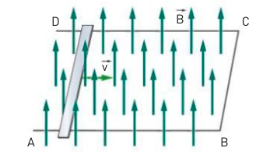
\includegraphics[width=0.9\textwidth]{images/circuito_U}
\end{minipage}
\begin{solution}
    \begin{enumerate}
        \item La sbarra in moto genera una f.e.m. mozionale, proporzionale alla lunghezza della sbarra e alla sua velocità:
        \[
        \mathcal{E} = B\,v\,l = 0{,}40\cdot 0{,}02\cdot 0{,}15 = \mathbf{1{,}2\times10^{-3}\ \text{V}} = 1{,}2\ \text{mV}.
        \]
        \item Dalla legge di Ohm:
        \[
        I = \frac{\mathcal{E}}{R} = \frac{1{,}2\times10^{-3}}{15} = \mathbf{8\times10^{-5}\ \text{A}} = 0{,}08\ \text{mA}.
        \]
    \end{enumerate}
\end{solution}
\end{question}

%------------------------------------------------%

\begin{question}[ID=1.9, subtitle={Orecchini circolari nel campo magnetico terrestre — flusso e f.e.m.}, tags={induzione magnetica, flusso}, difficulty=media]
Orecchini a cerchio di raggio $R = 2\ \text{cm}$; campo magnetico terrestre $B = 4\ \text{Gauss} = 4\times10^{-4}\ \text{T}$.
\vspace{10pt}

\begin{minipage}{0.7\textwidth}
    \begin{enumerate}
        \item Calcola il flusso del campo magnetico che attraversa perpendicolarmente la superficie.
        \item Dopo una rotazione di $90^\circ$, quanto vale il flusso?
        \item Se il movimento avviene in $\Delta t = 0{,}5\ \text{s}$, quanto vale la f.e.m. indotta?
    \end{enumerate}
\end{minipage}
\begin{minipage}{0.3\textwidth}
    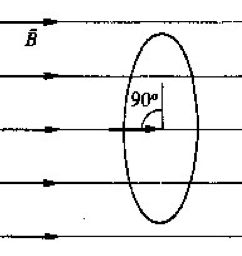
\includegraphics[width=0.7\textwidth]{images/flusso_spira_circolare}
\end{minipage}
\begin{solution}
    \begin{enumerate}
        \item L'area del cerchio è $A = \pi(0{,}02)^2 = 1{,}257\times10^{-3}\ \text{m}^2$. Con il campo perpendicolare alla superficie il flusso iniziale è
        \[
        \Phi_i = B\,A = 4\times10^{-4}\cdot 1{,}257\times10^{-3} \approx \mathbf{5{,}03\times10^{-7}\ \text{Wb}}.
        \]
        \item Dopo una rotazione di $90^\circ$ il campo giace nel piano della spira (parallelo alla superficie), quindi non la attraversa: $\Phi_f = \mathbf{0}$.
        \item La f.e.m. media è la variazione di flusso diviso il tempo impiegato:
        \[
        \mathcal{E}_{ind} = \frac{|\Delta\Phi|}{\Delta t} = \frac{5{,}03\times10^{-7}}{0{,}5} \approx \mathbf{1{,}0\times10^{-6}\ \text{V}} = 1{,}0\ \mu\text{V}.
        \]
    \end{enumerate}
\end{solution}
\end{question}


\begin{question}[ID=1.10, subtitle={Catena luminosa come solenoide — induttanza, corrente e costante di tempo}, tags={induzione magnetica, solenoide, circuito RL}, difficulty=difficile]
Una catena luminosa schematizzata come solenoide: $l = 15\ \text{cm}$, $R_{sol} = 5\ \text{cm}$, $N = 50$ spire, $R_{circ} = 2\ \Omega$, $\mathcal{E} = 12\ \text{V}$ (c.c.).
\begin{enumerate}
\item Calcola l'induttanza.
\item Calcola la corrente massima.
\item Calcola il flusso del campo magnetico.
\item Calcola la costante di tempo $\tau$.
\item Scrivi la legge $i(t)$.
\item Calcola la corrente dopo $\Delta t = 2\times10^{-4}\ \text{s}$.
\end{enumerate}
\begin{solution}
\begin{enumerate}
\item L'induttanza di un solenoide dipende dal numero di spire, dall'area e dalla lunghezza. Con $A = \pi(0{,}05)^2 = 7{,}854\times10^{-3}\ \text{m}^2$:
\[
L = \frac{\mu_0 N^2 A}{l} = \frac{4\pi\times10^{-7}\cdot 2500\cdot 7{,}854\times10^{-3}}{0{,}15} \approx \mathbf{1{,}645\times10^{-4}\ \text{H}}.
\]
\item A regime l'induttanza non limita la corrente, che vale per la legge di Ohm:
\[
I_{max} = \frac{\mathcal{E}}{R} = \frac{12}{2} = \mathbf{6\ \text{A}}.
\]
\item Il campo all'interno del solenoide è $B = \mu_0 N I_{max}/l = 4\pi\times10^{-7}\cdot 50\cdot 6/0{,}15 \approx 2{,}513\times10^{-3}\ \text{T}$, e il flusso concatenato con tutte le spire è
\[
\Phi = N\,B\,A \approx \mathbf{9{,}87\times10^{-4}\ \text{Wb}}.
\]
\item La costante di tempo del circuito RL è
\[
\tau = \frac{L}{R} = \frac{1{,}645\times10^{-4}}{2} \approx \mathbf{8{,}2\times10^{-5}\ \text{s}}.
\]
\item Durante il transitorio la corrente cresce esponenzialmente verso $I_{max}$:
\[
i(t) = 6\!\left(1 - e^{-t/\tau}\right)\ \text{A}.
\]
\item Sostituendo $\Delta t = 2\times10^{-4}\ \text{s}$ (cioè $t/\tau \approx 2{,}43$):
\[
i(2\times10^{-4}) = 6\,(1 - e^{-2{,}43}) \approx 6\cdot 0{,}912 \approx \mathbf{5{,}47\ \text{A}}.
\]
\end{enumerate}
\end{solution}
\end{question}

\begin{question}[ID=1.11, subtitle={Circuito RL chiuso e poi aperto — correnti in funzione del tempo}, tags={induzione magnetica, circuito RL}, difficulty=difficile]
Circuito RL: $\Delta V = 20\ \text{V}$, $R = 4{,}2\ \Omega$, $L = 2{,}5\ \text{H}$. Chiuso per $0{,}7\ \text{s}$, poi aperto.
\begin{parts}
\vspace{5pt}
\begin{minipage}{\linewidth}

\begin{wrapfigure}{r}{0.3\textwidth}
    \vspace{-20pt}
    \centering
    \includegraphics[width=0.3\textwidth]{circuito-rl}
\end{wrapfigure}
\part Calcola la costante di tempo.
\part Corrente massima nel circuito.
\part Corrente dopo $0{,}5\ \text{s}$ dall'apertura.
\part Dopo quanto tempo l'intensità è il $10\%$ della corrente massima.
\part Descrivi qualitativamente e rappresenta la corrente in funzione del tempo.
\end{minipage}
\end{parts}
\begin{solution}
\begin{enumerate}
    \item La costante di tempo del circuito è
    \[
    \tau = \frac{L}{R} = \frac{2{,}5}{4{,}2} \approx \mathbf{0{,}595\ \text{s}}.
    \]
    \item La corrente massima (a regime) è data dalla legge di Ohm:
    \[
    I_{max} = \frac{\Delta V}{R} = \frac{20}{4{,}2} \approx \mathbf{4{,}76\ \text{A}}.
    \]
    \item Al momento dell'apertura ($t = 0{,}7\ \text{s}$) il circuito non ha ancora raggiunto $I_{max}$: la corrente vale $I_0 = I_{max}(1 - e^{-0{,}7/0{,}595}) \approx 4{,}76\cdot 0{,}692 \approx 3{,}29\ \text{A}$. Dopo l'apertura la corrente decade esponenzialmente, $I(t') = 3{,}29\,e^{-t'/\tau}$, e a $t' = 0{,}5\ \text{s}$:
    \[
    I = 3{,}29\,e^{-0{,}840} \approx \mathbf{1{,}42\ \text{A}}.
    \]
    \item Imponendo $I(t') = 0{,}1\,I_{max} = 0{,}476\ \text{A}$ nella legge di decadimento:
    \[
    t' = \tau\ln\!\frac{3{,}29}{0{,}476} = 0{,}595\cdot\ln(6{,}91) \approx \mathbf{1{,}15\ \text{s}}.
    \]
    \item Durante la fase di chiusura la corrente cresce esponenzialmente verso $I_{max}$ con costante di tempo $\tau$; dopo l'apertura decade esponenzialmente verso zero con la stessa costante di tempo. Il grafico è quindi una curva crescente «a saturazione» seguita da una curva di decadimento.
\end{enumerate}
\end{solution}
\end{question}
